\documentclass[../main.tex]{subfiles}
\graphicspath{{\subfix{../images/}}}
\begin{document}
\section*{Term 2 Week 5}
\begin{enumerate}
    \item 
    Start by zooming in on one section of the hexagon:
    \begin{figure}[H]
        \centering
        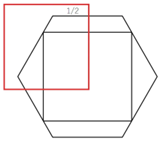
\includegraphics[width=0.25\linewidth]{images/t2w5q1_a1.png}
    \end{figure}
    Assume that each side of the square has length \(2x\). We also split the side length of the hexagon into two sections either side of the vertex of the square, giving us lengths of \textit{a} and \(1-a\).
    \begin{figure}[H]
        \centering
        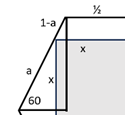
\includegraphics[width=0.25\linewidth]{images/t2w5q1_a2.png}
    \end{figure}
    Since the interior angles of a regular hexagon are 120\(^{\circ}\), we get:\\
    \(\sin{60}=\frac{x}{a}\)\\
    \(x=a \sin{60}=\frac{\sqrt{3}}{2}a\)\\
    \(a=\frac{2}{\sqrt{3}}x\)\\

    Also, the angle at the top of the small triangle will be 30\(^{\circ}\). This means that the base of that triangle will be \(\frac{1-a}{2}\).\\
    This gives us \(x-\frac{1-a}{2}=\frac{1}{2}\)\\
    Rearranging:\\
    \(2x-1+a=1\)\\
    \(2x+a=2\)\\

    Substituting in from the other equation:\\
    \(2x+\frac{2}{\sqrt{3}}x=2\)\\

    Solving for \textit{x}:\\
    \(2\sqrt{3}x+2x=2\sqrt{3}\)\\
    \(x(2\sqrt{3}+2)=2\sqrt{3}\)\\
    \(x=\frac{2}{2\sqrt{3}+2}=\frac{\sqrt{3}}{\sqrt{3}+1}\)\\

    Rationalising:\\
    \(x=\frac{\sqrt{3}}{\sqrt{3}+1}\times \frac{\sqrt{3}-1}{\sqrt{3}-1}=\frac{3-\sqrt{3}}{2}\)\\

    Side length of square \(=2x=3-\sqrt{3}\)\\
    Area of square \(=(3-\sqrt{3})(3-\sqrt{3})=12-6\sqrt{3}\)\\

    \item 
    First rewrite as \(y=x^y\)\\

    Take the natural log of both sides:\\
    \(\ln{y}=\ln{(x^y)}\)\\
    \(\ln{y}=y\ln{x}\)\\

    Differentiate implicitly, don't forget the Product Rule.\\
    \(\frac{1}{y}\frac{dy}{dx}=\ln{x}\frac{dy}{dx}+\frac{y}{x}\)\\

    Rearrange:\\
    \(\frac{1}{y}\frac{dy}{dx}-\ln{x}\frac{dy}{dx}=\frac{y}{x}\)\\
    \((\frac{1}{y}-\ln{x})\frac{dy}{dx}=\frac{y}{x}\)\\
    \((\frac{1-y\ln{x}}{y})\frac{dy}{dx}=\frac{y}{x}\)\\
    \(\frac{dy}{dx}=\frac{y^2}{x(1-y\ln{x})}\)\\

    Optionally, substitute back in for \textit{x}:\\
    \(\frac{dy}{dx}=\frac{(x^{x^{x^{x^{.^{.^{.}}}}}})^2}{x(1-x^{x^{x^{x^{.^{.^{.}}}}}}\ln{x})}\)\\

    \item 
    \(a-1=\frac{x}{y}\) and \(b-1=\frac{y}{x}\).\\
    This means that \(a-1=\frac{1}{b-1}\)\\

    \((a-1)(b-1)=1\)\\
    \(ab-a-b+1=1\)\\
    \(ab=a+b\)\\

    \((a+b)^2=a^2+b^2+2ab\)\\
    \((a+b)^2=15+2ab\)\\
    \((a+b)^2-2ab-15=0\)\\

    Remember \(ab=a+b\), therefore we can make a substitution and solve a quadratic.\\
    \((ab)^2-2ab-15=0\)\\
    \(ab=5,-3\)\\

    Since \textit{a} and \textit{b} are positive, we know \(ab=a+b=5\).\\

    \((a+b)^3=a^3+3a^2b+3ab^2+b^3=125\)\\
    \(a^3+b^3=125-3a^2b-3ab^2\)\\
    \(a^3+b^3=125-3ab(a+b)\)\\

    And since \(ab=a+b=5\), \(a^3+b^3=125-3\times 5 \times 5=50\)\\    

    \item 
    Since the left-hand side is an even function (symmetrical about the y-axis), it means that for every \(x\) that solves the equation, \(-x\) will also be a solution. If we pair the solutions up, the sum must be zero.
     
    \end{enumerate}

\end{document}